%%
%% Copyright 2007-2019 Elsevier Ltd
%%
%% This file is part of the 'Elsarticle Bundle'.
%% ---------------------------------------------
%%
%% It may be distributed under the conditions of the LaTeX Project Public
%% License, either version 1.2 of this license or (at your option) any
%% later version.  The latest version of this license is in
%%    http://www.latex-project.org/lppl.txt
%% and version 1.2 or later is part of all distributions of LaTeX
%% version 1999/12/01 or later.
%%
%% The list of all files belonging to the 'Elsarticle Bundle' is
%% given in the file `manifest.txt'.
%%

%% Template article for Elsevier's document class `elsarticle'
%% with numbered style bibliographic references
%% SP 2008/03/01
%%
%%
%%
%% $Id: elsarticle-template-num.tex 168 2019-02-25 07:15:41Z apu.v $
%%
%%
\documentclass[preprint,3p,times]{elsarticle}

%% Use the option review to obtain double line spacing
%% \documentclass[authoryear,preprint,review,12pt]{elsarticle}

%% Use the options 1p,twocolumn; 3p; 3p,twocolumn; 5p; or 5p,twocolumn
%% for a journal layout:
%% \documentclass[final,1p,times]{elsarticle}
%% \documentclass[final,1p,times,twocolumn]{elsarticle}
%% \documentclass[final,3p,times]{elsarticle}
%% \documentclass[final,3p,times,twocolumn]{elsarticle}
%% \documentclass[final,5p,times]{elsarticle}
%% \documentclass[final,5p,times,twocolumn]{elsarticle}
% \usepackage[american]{babel}
\usepackage{mdframed}
\usepackage{microtype}
\usepackage{xcolor}
\usepackage{multirow}
\usepackage{amsmath}
\usepackage{amsfonts}
\usepackage{graphicx}
\usepackage{booktabs}
\usepackage{subfig}
\usepackage{array}
\usepackage{tabularx}
\usepackage{dsfont}
\usepackage{float}
\usepackage{amsthm}
\usepackage{float}
\usepackage[normalem]{ulem}
\usepackage[mathscr]{euscript}
\newcolumntype{Y}{>{\centering\arraybackslash}X}

\definecolor{redunknown}{RGB}{239, 68, 112}
\definecolor{blueknown}{RGB}{38, 171, 227}

\newcommand\knowncolor[1]{\textcolor{blueknown}{#1}}
\newcommand\unknowncolor[1]{\textcolor{redunknown}{#1}}

\newmdenv[
  topline=false,
  bottomline=false,
  skipabove=\topsep,
  skipbelow=\topsep,
  leftmargin=20pt,
  rightmargin=20pt,
  innertopmargin=5pt,
  innerbottommargin=5pt
]{siderules}

% \setlength{\jot}{10pt}

\usepackage[ruled,norelsize]{algorithm2e}



%% For including figures, graphicx.sty has been loaded in
%% elsarticle.cls. If you prefer to use the old commands
%% please give \usepackage{epsfig}

%% The amssymb package provides various useful mathematical symbols
\usepackage{amssymb}
%% The amsthm package provides extended theorem environments
%% \usepackage{amsthm}

%% The lineno packages adds line numbers. Start line numbering with
%% \begin{linenumbers}, end it with \end{linenumbers}. Or switch it on
%% for the whole article with \linenumbers.
%% \usepackage{lineno}

\renewcommand{\theequation}{R2.\arabic{equation}}

\makeatletter
\renewcommand{\MaketitleBox}{%
  \resetTitleCounters
  \def\baselinestretch{1}%
  \begin{center}
    \def\baselinestretch{1}%
    \Large \@title \par
    \vskip 18pt
    \normalsize \par
    \vskip 10pt
    \footnotesize \itshape  \par
  \end{center}
  \vskip 12pt
}
\makeatother

\makeatletter
\def\ps@pprintTitle{%
 \let\@oddhead\@empty
 \let\@evenhead\@empty
 \def\@oddfoot{\centerline{\thepage}}%
 \let\@evenfoot\@oddfoot}
\makeatother

% \setlength{\parindent}{4em}
\setlength{\parskip}{0.8em}

\begin{document}
\begin{frontmatter}
    \title{Reply to Reviewer\#2}
\end{frontmatter}

\renewcommand{\figurename}[1]{Fig.R2.#1}
%% \linenumbers

%% main text
% \section{aa}
\section*{In the main idea, it is not clear the sampling proportion between the data from known and unknown classes. How does this proportion affect the subsequent training?}

\subsection*{\underline{\textbf{Response:}}}

As you mentioned, it’s essential to indicate the affection of samples from unknown classes in the setting of open set domain adaptation. 
However, in real scenarios, we can not manually set the sampling proportion due to the lack of target label information.
During the training phase, ThDAN is confined to randomly sample training data from the target domain.
So we conduct experiments to implicitly change the sampling proportion by varying the number of unknown data and the number of unknown classes.
All experiments are conducted on Office-31 datasets.
Results show as follows,
\begin{figure*}[htb]
    \centering
    \subfloat[\footnotesize Accury \textit{w.r.t.} number of classes that are treated as the unknown]{
        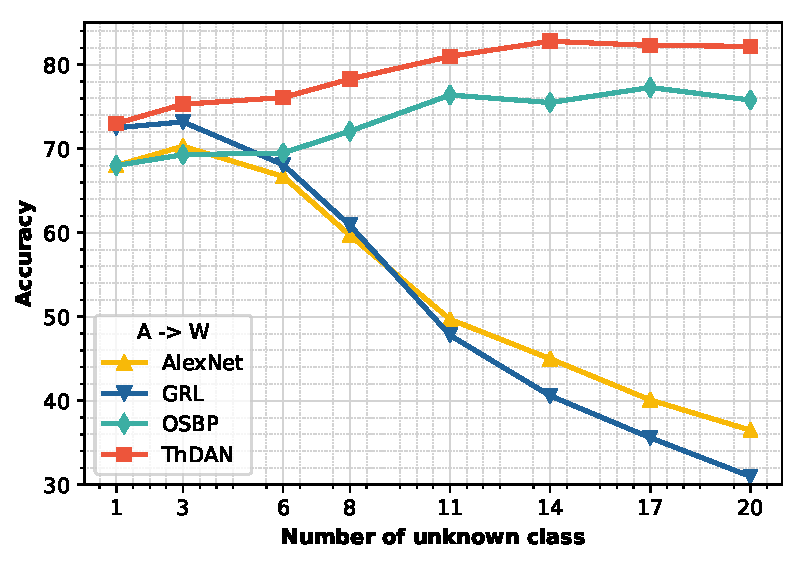
\includegraphics[width=0.33\textwidth]{contents/figures/pdf/analysis/class_change.pdf} 
        \label{figure: number of unknown class f}
    }
    \subfloat[\footnotesize Accury \textit{w.r.t.} ratio of used unknown samples]{
        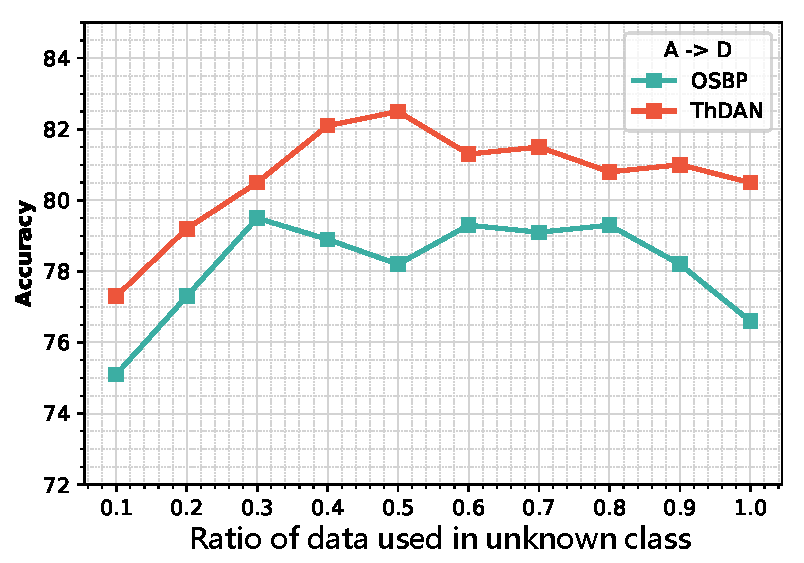
\includegraphics[width=0.34\textwidth]{contents/figures/pdf/analysis/nuknown_change.pdf} 
        \label{figure: ration of unknown f}
    } 
    \\
    \caption{
        (\textbf{a}): 
        The accuracy when we change the ratio of unknown samples in the adaptation task \textit{A$\to$D}. 
        (\textbf{b}): 
        The accuracy when we change the number of classes that are treated as the unknown in the adaptation task \textit{A$\to$W}. 
    }
    \label{figure: analysis change ratio}
\end{figure*}


We first fix the number of unknown classes to 10, and then change the sample number of each unknown class.
\textbf{Ratio 0.1} of sample number indicates that only one-tenth samples of each unknown class are used for training and testing, while the others are discarded from the dataset.
\figurename{\ref{figure: ration of unknown f}} shows the result.
When the ratio is low, the model can hardly identify samples from unknown classes due to lack of training samples. 
On the contrary, when the ratio is high, the negative transfer of unknown class would undermine the classification of the known class. 
Therefore the performance of the model is defective around the endpoint of the interval. 

We further vary the number of unknown classes in \figurename{\ref{figure: number of unknown class f}}. 
As the number of unknown classes increases, the performance of the methods proposed for close set domain adaptation will decrease significantly. 
That is because they cannot alleviate the negative transfer brought by the unknown classes.
The model proposed for open set domain adaptation would gains performance improvement by correctly rejecting samples from unknown classes. 
That is because it's easier to reject samples as the ``unknown'' than categorize samples from the diverse known classes.  
The accuracy has the trend to decay since too many unknown classes would interfere with the model on classifying the known class.

The experiments show that the sampling proportion between the data from known and unknown classes could substantially affect model training for both known and unknown classes. 
Low proportion of sample from unknown classes would affect the discrimination of unknown samples, and high proportion of that would undermine classifications of samples from known classes. 

\section*{From their reported results in \textcolor{blue}{Figure 7}, the adjust threshold of $\gamma_0$ is not sensitive to the accuracy of training, it is a bit strange.  Authors are encouraged to carefully check their claims by using more detailed reasons or more diverse data sets. }

\subsection*{\underline{\textbf{Response:}}}

Thanks for your suggestions.
In our model, the threshold is calculated by averaging the transferability score of a batch of source samples and the predefined $\gamma$ as follows,
\begin{equation}
    \label{eq: transferability thresholded}
    \beta(X_s, \gamma) = \mathbb{E}_{x \in X_s} w(x) - \gamma.
\end{equation}

Then we dynamically increase $\gamma$ from $0$ to $\gamma_0$ so that more samples could be selected for adversarial training. 
The changing function of $\gamma$ as follows,
\begin{equation}  
    \label{eq: dynamic tolerable range}
    \begin{split}
        \gamma &= 
        \begin{cases}
            0 & ,\: n \in N_1 \\
            \gamma_0 \times  \sigma(n) & ,\: n\in N_2 \\ 
        \end{cases}
    \end{split}
\end{equation}
where $\gamma$ is a \textit{monotonically increasing function} with an upper bound of $1$. 

In experiments, we verify that the model is insensitivity to the value of $\gamma_0$ on \textbf{6 tasks of Office-31} and \textbf{12 tasks of Office-Home}. 
We include \textcolor{blue}{Figure7} of the original paper as follows, which shows the average prediction accuracy on these datasets when $\gamma_0$ varies,
\begin{figure}[htb]
    \centering
    \subfloat[Accury \textit{w.r.t.} the value of $\gamma_0$]{
        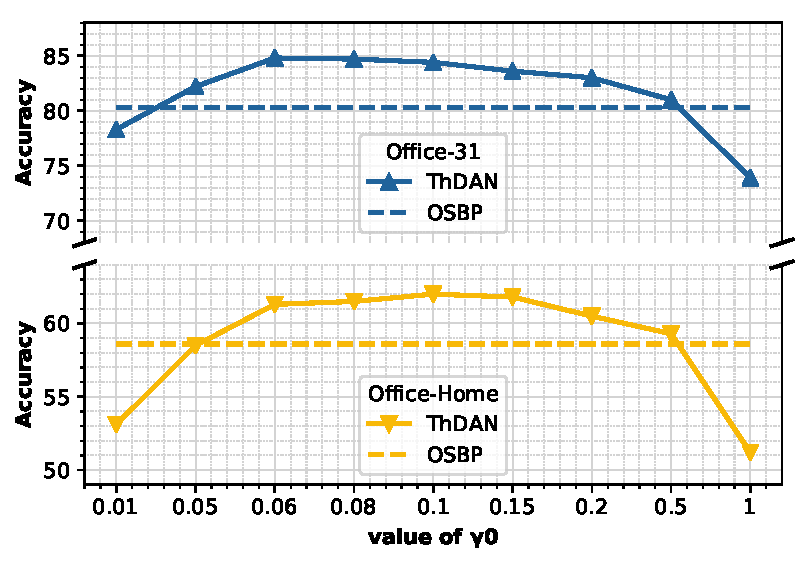
\includegraphics[width=0.33\textwidth]{contents/figures/pdf/analysis/sigma_change.pdf} 
        \label{figure: analysis in question 2}
    }
    \\
    \caption{
        The prediction accuracy of our method when we change the value of $\gamma_0$ on dataset Office-31 and Office-Home. 
    }
\end{figure}

Compared with the baseline model OSBP, our model can deliver plausible results on both Office-31 and Office-Home datasets when the $\gamma_0$ in the range of $[0.06, 0.5]$. 
That is because when we gradually increase the $\gamma$ during training, we also gradually decrease the learning rate. 
As a result, the transferable samples selected in early stage would ‘dominate’ the model training, because they engage in training sooner, and the gradient produced by them can update the model with a greater learning rate. 
As the $\gamma$ approaches $\gamma_0$, the learning rate is relatively small, and the previously selected samples would still be selected for training, thus the newcomer has little impact on model performance. 
This directly reflects on the insensitivity of value of $\gamma_0$ to the accuracy of training. 

The above explanation has been added in the revised manuscript. 
Please refer to Section 4.3.6 in the revised manuscript for details.


\section{
    The abstract needs to be redesigned. 
    Open set domain adaptation (OSDA) should be a scenario. 
    Authors claim to solve the OSDA problem. What is the problem?? This is unclear. 
    It seems the author should firstly explain the OSDA setting and then present which issue they want to address. The first sentence of the abstract is a bit far away from their focus. 
    More seriously, the introduction don not connect the abstract. 
    For example, the beginning of the abstract explains the unsupervised domain adaptation, but the beginning of the introduction suddenly use deep learning to start this paper without unsupervised domain adaptation. 
    Authors are encouraged to carefully reorganize their work, where the introduction must connect the abstract tightly. 
    One sentence in the abstract should connect one logic in the introduction section. 
}

\subsection*{\subsection*{\underline{\textbf{Response:}}}}



Thanks for your precious suggestions, which is very helpful for us in improving paper writing.
The \textbf{abstract}, \textbf{introduction} and \textbf{method} sections of revised manuscript have been reorganized for tighter logical connections.

The \textbf{abstract} has being redesigned as follows,
\begin{siderules}
    \textit{
        \footnotesize
        Unsupervised domain adaptation (UDA) is a paradigm to tackle domain shift problem.
        Most existing UDA methods are proposed for Close Set Domain Adaptation (\textit{CSDA}) which assumes source and target domains share the same label space.
        More practically, target domain contains unknown class different from the known ones in the source domain, i.e., Open Set Domain Adaptation (\textit{OSDA}).
        Due to the presence of unknown classes, aligning the whole distribution of the source and target domain for OSDA as in the previous method will lead to negative transfer. 
        Existing methods developed for OSDA try to assign smaller weights to target samples of unknown class.
        Despite promising performance, the samples of unknown class are still used for training, which exposes the model to the risk of negative transfer.
        Instead of reweighting, this paper presents a novel method namely Thresholded Domain Adversarial Network (\textit{ThDAN}), which progressively selects transferable target samples for distribution alignment. 
        Based on the fact that samples from the known classes must be more transferable than target samples of the unknown one, we derive a criterion to quantify the transferability by constructing classifiers to categorize known classes and to discriminate unknown class.
        In ThDAN, an adaptive threshold is calculated by averaging transferability scores of source domain samples to select target samples for training. 
        The threshold is tweaked progressively during the training process so that more and more target samples from the known classes can be correctly selected for adversarial training.
        Extensive experiments show that the proposed method outperforms state-of-the-art domain adaptation and open set recognition approaches on benchmarks.
    }
\end{siderules}
In the revised abstract, we first introduce the unsupervised domain adaptation (UDA).
Then we make an introduction to the open set domain adaptation (OSDA) and the challenge of it.
To clarify the motivation of our work, we then introduce the working mechanism of existing models proposed for OSDA and state the drawbacks of it.
Finally, we present the general idea of the proposed Thresholded Domain Adversarial Network (ThDAN).

Following the logic of the redesigned abstract, we modified the \textbf{introduction} to make it more tightly connected to the abstract.
For example, in the first paragraph of the introduction, we first introduce the domain shift problem, then lead to the topic of unsupervised domain adaptation, which is logically related to the first sentence of the abstract. 

We also reorganized the subsections of \textbf{Method} section to make it more logical.
In the revised manuscript, a section of the introduction of domain adversarial training \cite{DomainAdversrialNetwork} is added as the preliminary of the proposed model.
Then in the next section, we introduce the general idea and training procedure of the proposed ThDAN.
In the following sections, we detailed introduce the transferability based sample selection algorithm used in ThDAN.
We consider such an organization can help readers better understand our work.

Please refer to Abstract, Section 1 and 3 in the revised manuscript for details.


\section{
    What is "transferable"? How to evaluate it? Any definition to support this term?
}
\label{question: transferable}

\subsection*{\underline{\textbf{Response:}}}


Unfortunately, there is no formal definition or mathematical formula to define ``transferable'' in the context of domain adaptation. 
Generally, the word ``transferable' is used to describe features. 
Here we quote from \cite{DeepAdaptationNetworks}:
\begin{quote}
    \textit{the transferable features are the features that generalize well to novel tasks for domain adaption}
\end{quote}
While the later work \cite{TransferableAttentionDA} uses ``transferable'' to describe samples that contribute to the transfer task of domain adaptation. 

In the scenario of open set domain adaptation, we consider the target samples from the known classes are transferable samples since they can boost the classification performance of the model.  
On the contrary, the target samples from the unknown classes are considered as untransferable samples, that is because aligning distribution with them will incur negative transfer. 

In this work, we evaluate transferability based on two observations:

\textbf{Target samples from the known classes are able to confuse $G_d$.} 
Here $G_d$ is the domain discriminator that gives the probability of being target samples.
For a target sample, if $G_d^*(z)$ approaches to $1$, then the sample has a high probability of coming from the unknown classes.
That is because the unknown classes only included in the target domain and can be almost perfectly discriminated from the source samples. 
On the other hand, if $G_d^*(z)$ approaches to $0$, then the sample is more likely from the known classes that shared by domains. 
Therefore, the transferable target samples are able to confuse $G_d$ to label them as the source samples.
Then we can define the transferability $w_d(x)$ as inversely related to $G_d^*(z)$ as ,
\begin{align}
    w_d(x) &= 1-G_d^*(z). \label{eq: domain transferability} 
\end{align}

\textbf{Target samples from the known classes can be categorized by $G_{c, known}$.}
Here $G_{c, known}$ is the classifier that gives the probability distribution among known classes.
Due to the overlapping in the marginal distributions, the target samples from the known classes should be categorized by the classifier $G_c$ that trained on the source samples, leading to low classification entropy.
And for samples from the unknown classes, because they cannot be aligned with a specific class from the source domain, the prediction tends to be uncertain over $K$ known categories, leading to high classification entropy.
Therefore the transferability $w_c(x)$ can be defined as inversely related to the \textit{normalized} classification entropy $H$ as,
\begin{align}
    w_c(x) &=1-H(G_{c,\; known}(z)). \label{eq: class transferability}
\end{align}

Since the domain discriminate $G_d$ in Eq.\ref{eq: domain transferability} and the classifier $G_{c, known}$ in Eq.\ref{eq: class transferability} work independently, we can unify the transferability criterion as,
\begin{equation}
    \label{eq: transferability}
    w(x)=1-G_d(z)\cdot H(G_{c,\; known}(z)).
\end{equation} 
The experiments in Section4 show that the transferability criterion of Eq.\ref{eq: transferability} works well for our model to select target samples from the known classes.


\section{
    In \textcolor{blue}{Figure1}, it is unclear why (d) must outperform the other methods. 
}

\subsection*{\underline{\textbf{Response:}}}


Thanks for your comments. 
The \textcolor{blue}{Figure1} in the original manuscript is as follows,

\begin{figure}[H]
    \centering
    \subfloat{
        
\includegraphics[width=0.55\textwidth]{contents/figures/pdf/overview/note.pdf} 
    }
    \\
    \addtocounter{subfigure}{-1}
    \subfloat[]{
        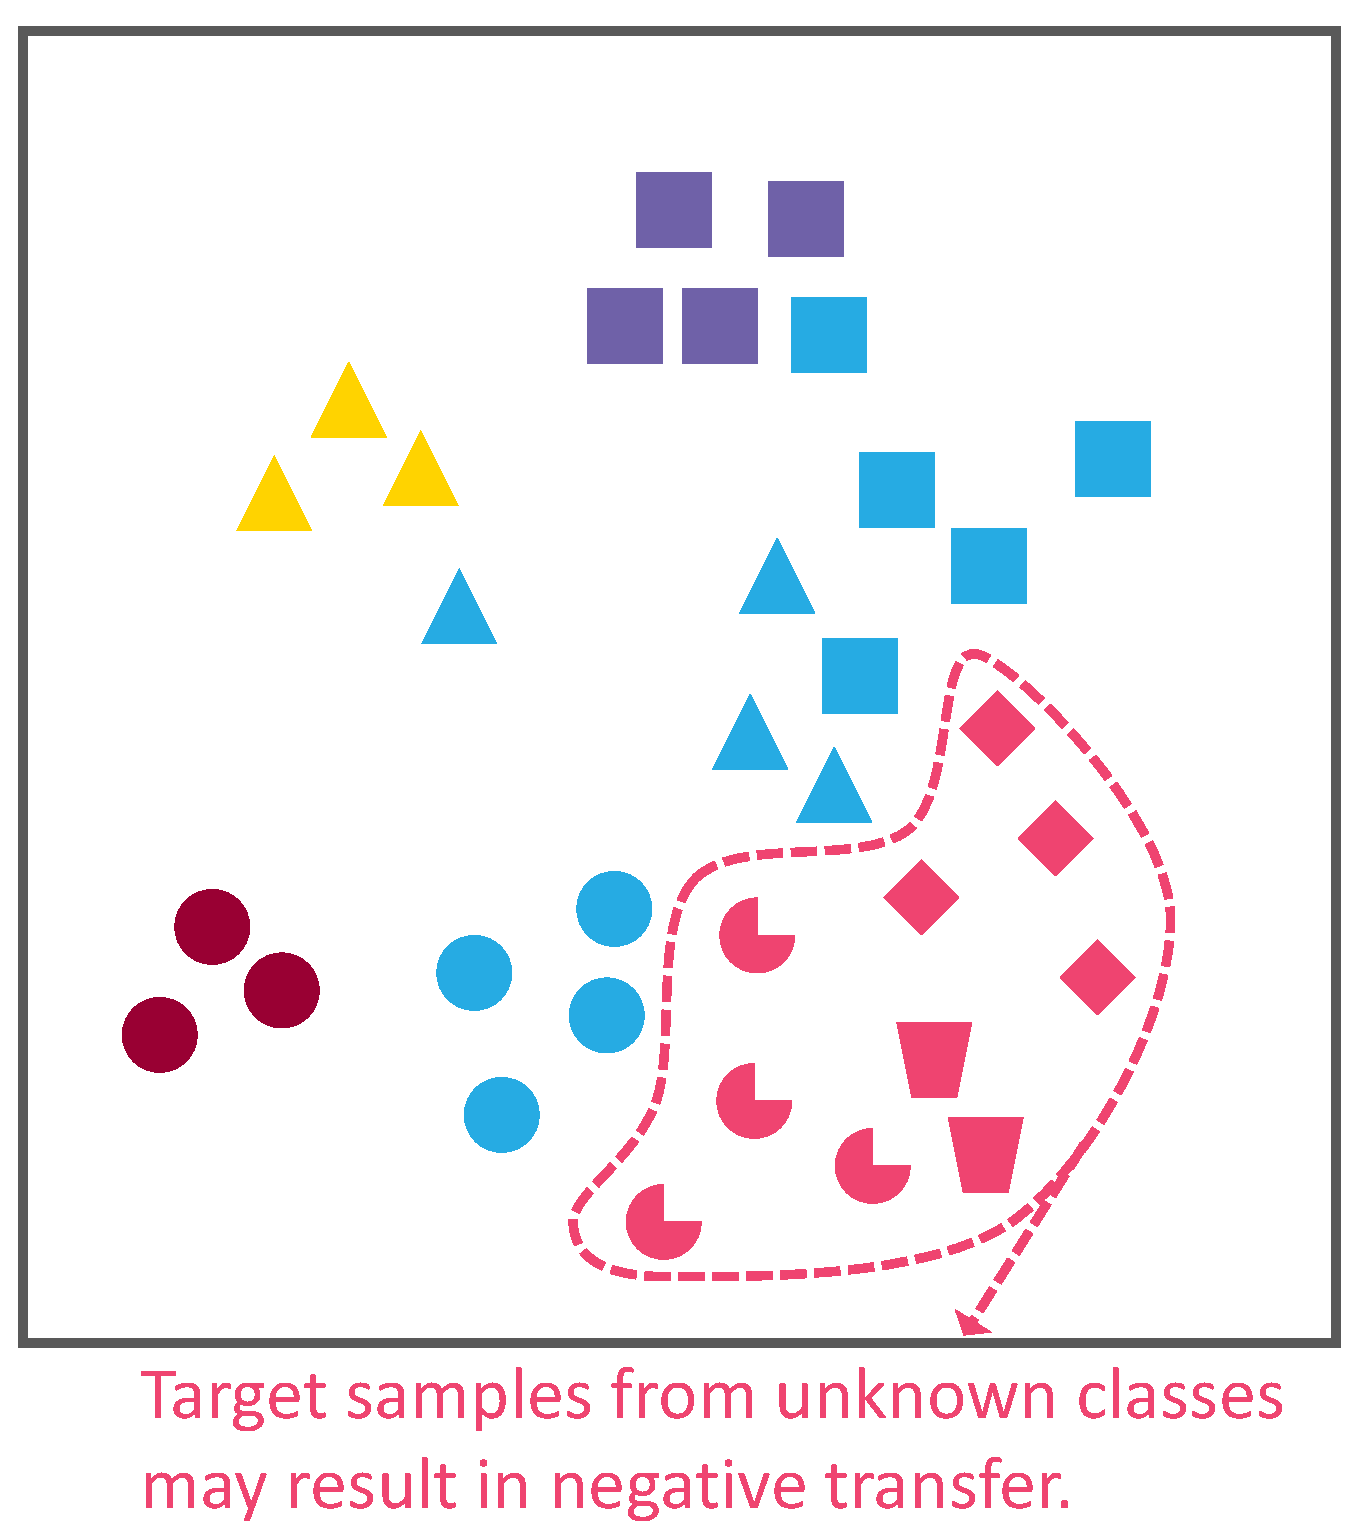
\includegraphics[width=0.22\textwidth]{contents/figures/pdf/overview/1.pdf} 
        \label{figure: reweighting based}
    } 
    \subfloat[]{
        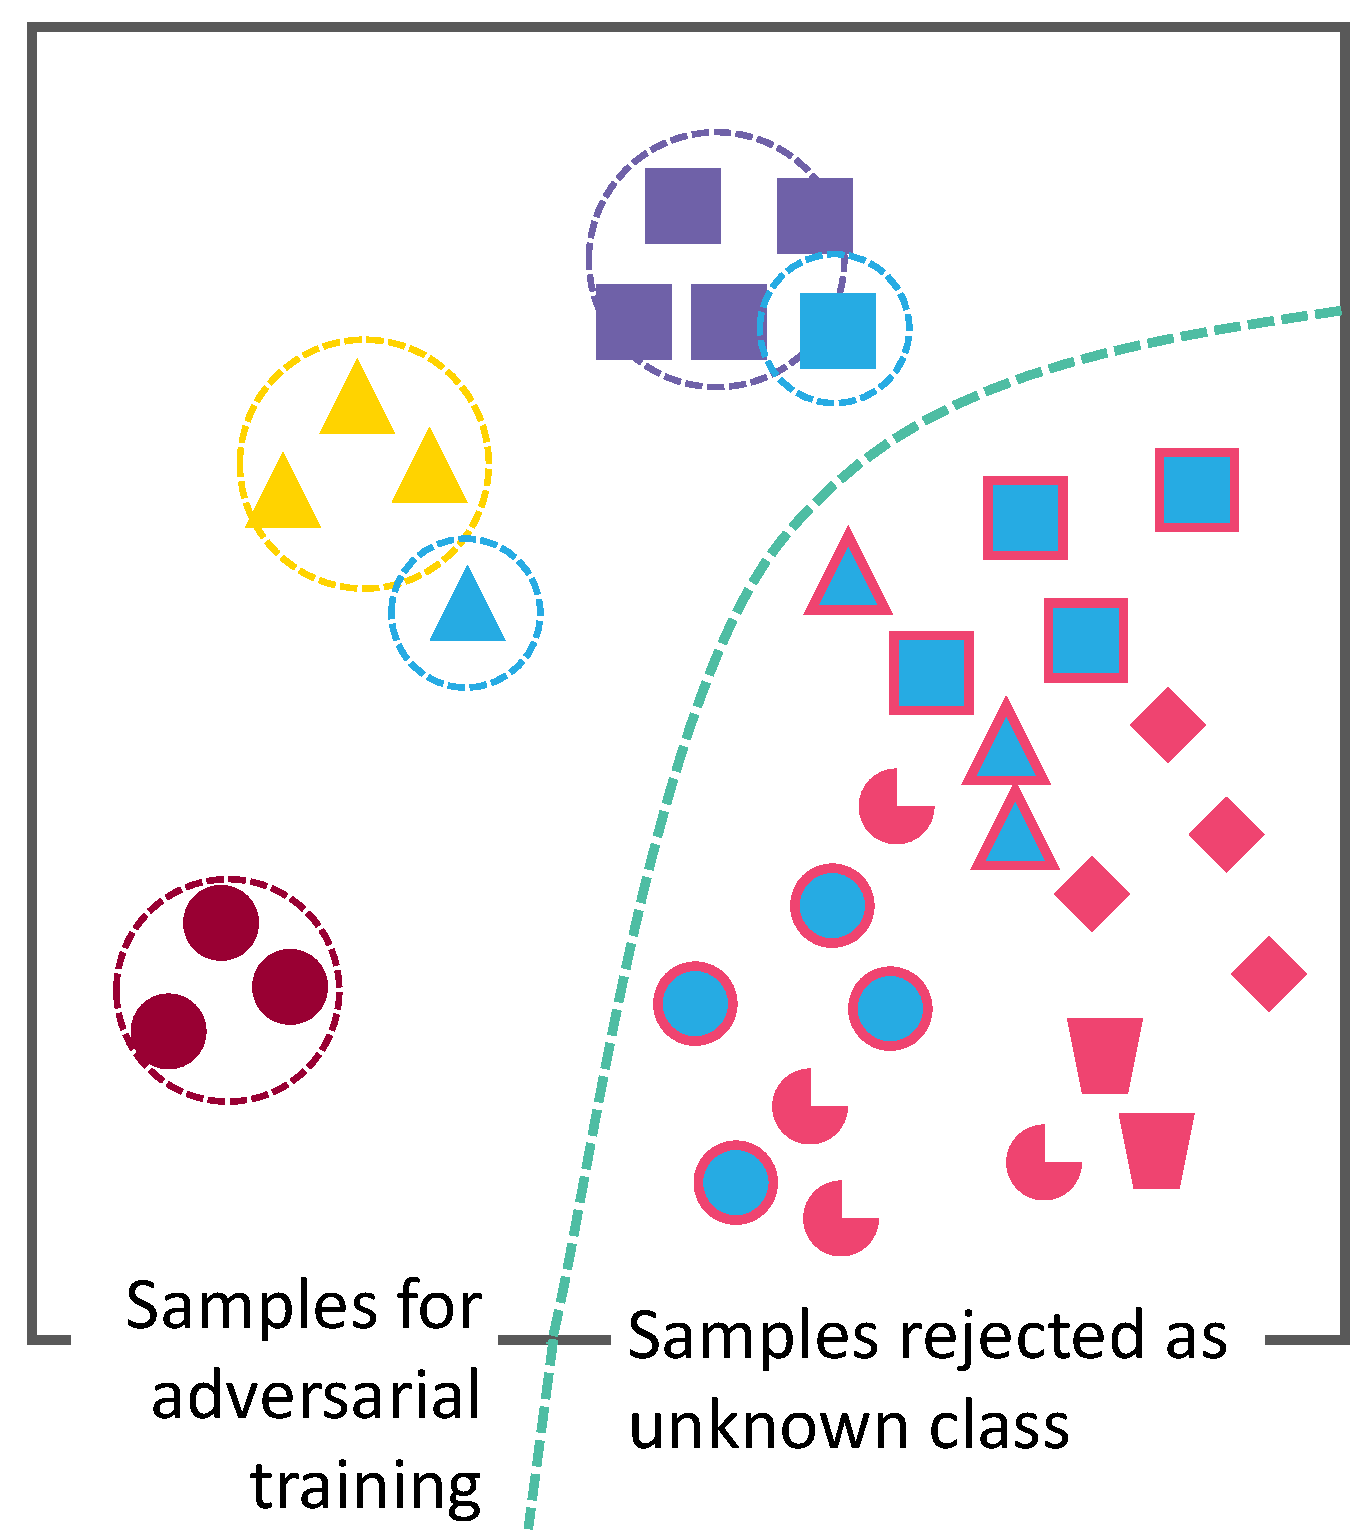
\includegraphics[width=0.22\textwidth]{contents/figures/pdf/overview/2.pdf} 
        \label{figure: ThDAN 1}
    } 
    \subfloat[]{
        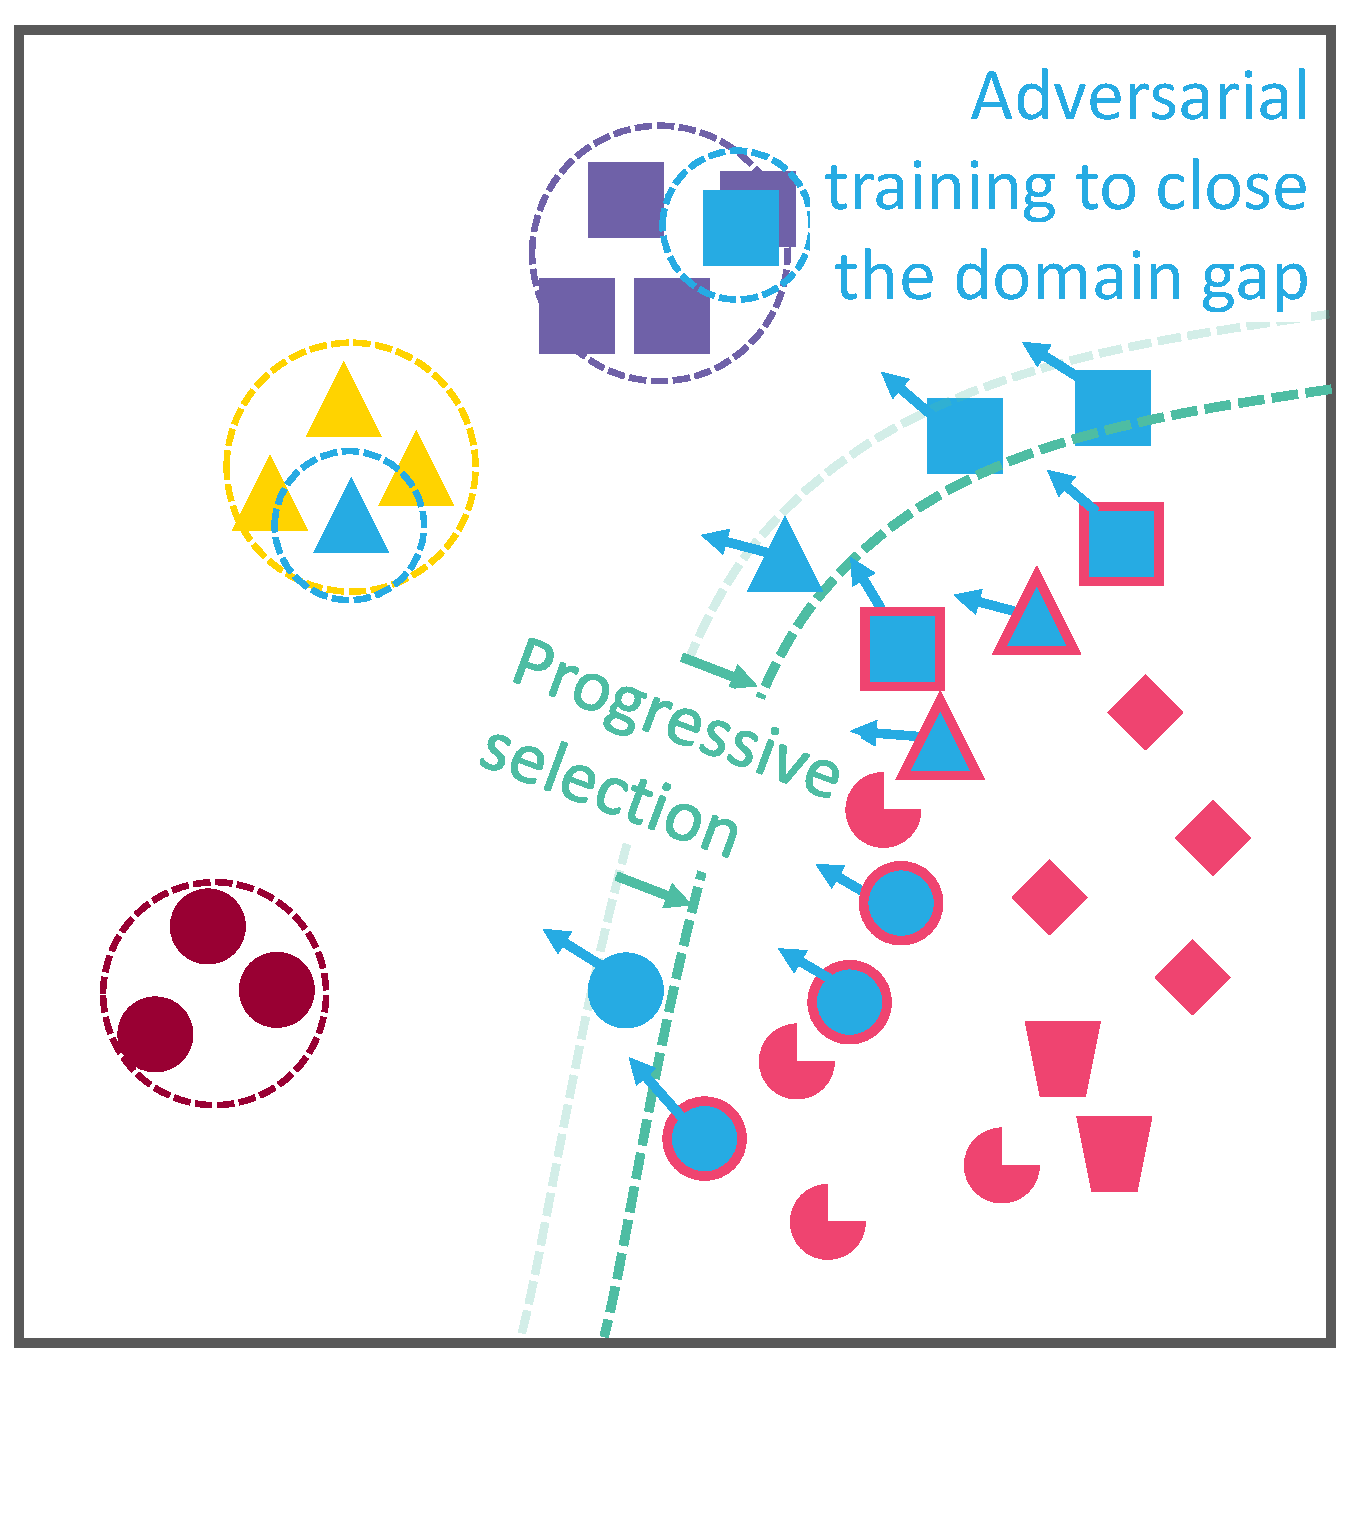
\includegraphics[width=0.22\textwidth]{contents/figures/pdf/overview/3.pdf} 
        \label{figure: ThDAN 2}
    } 
    % \hfil
    \subfloat[]{
        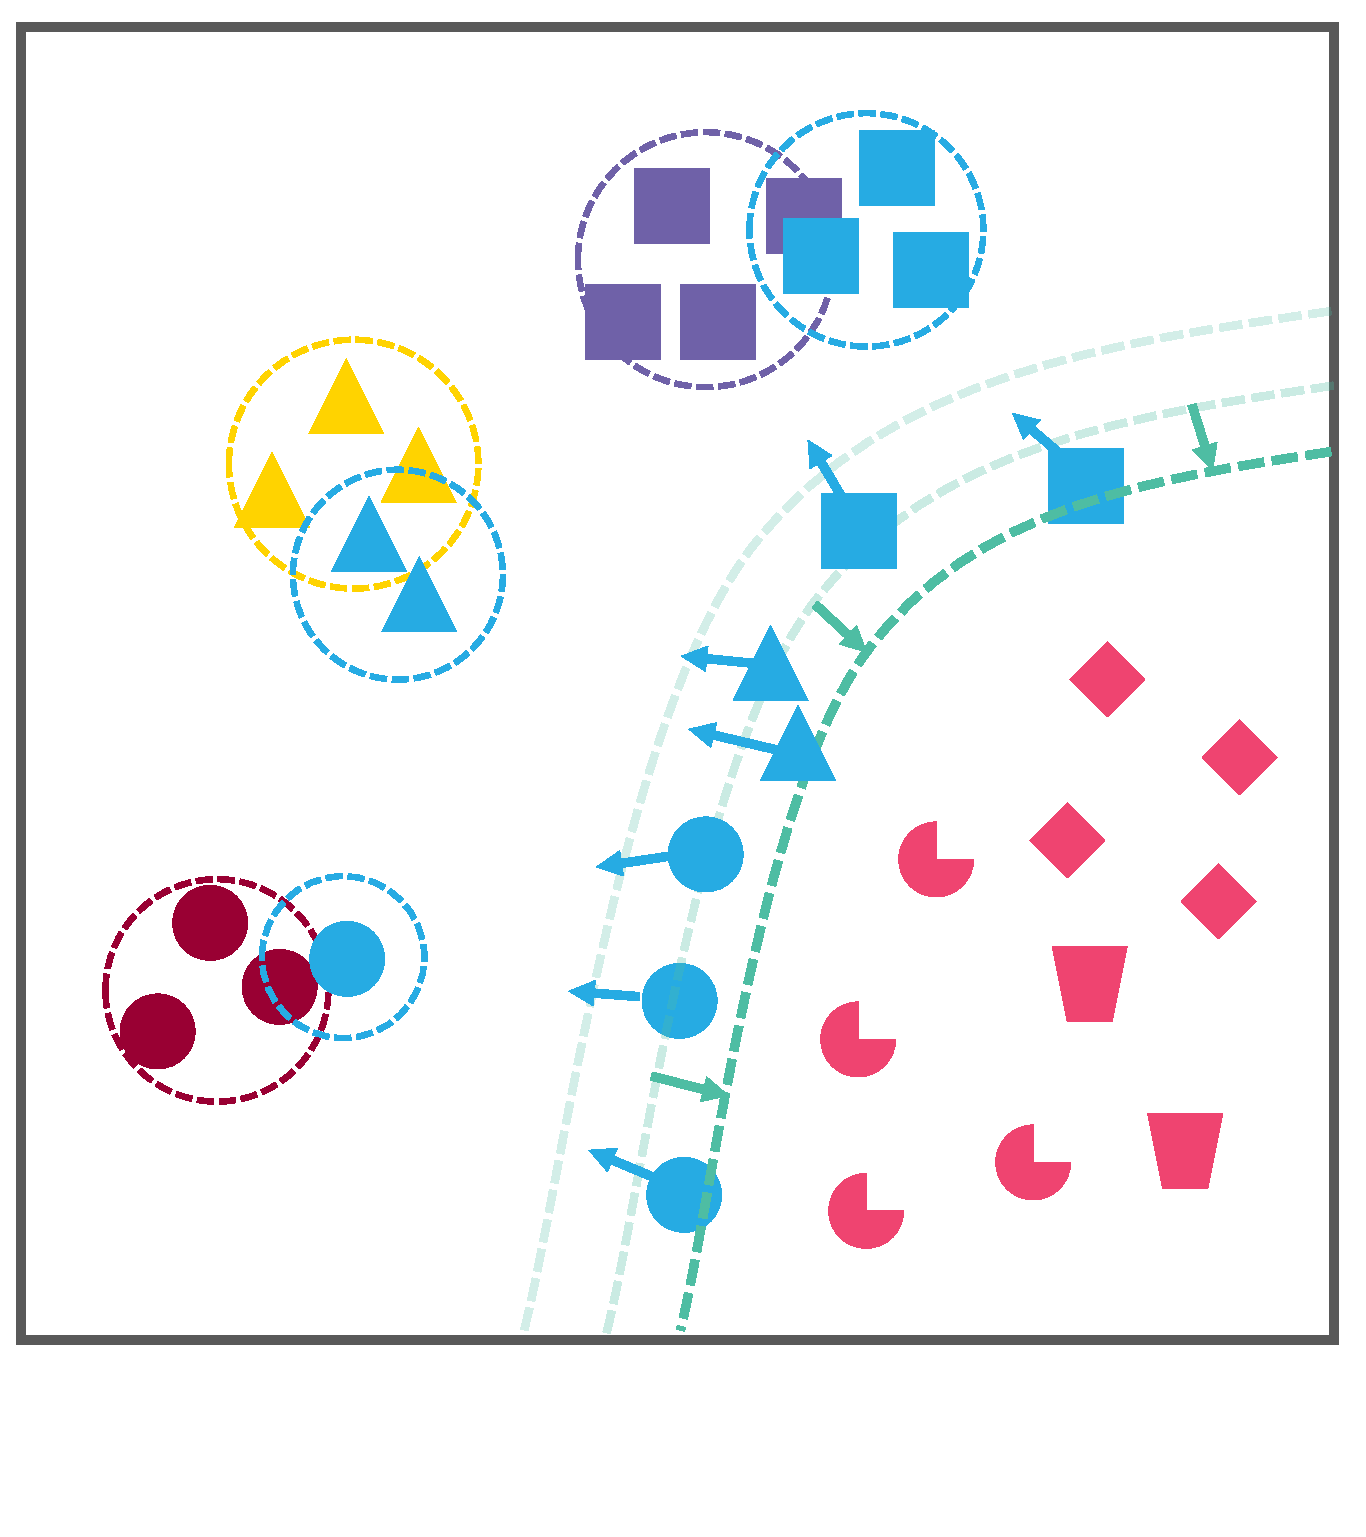
\includegraphics[width=0.22\textwidth]{contents/figures/pdf/overview/4.pdf} 
        \label{figure: ThDAN 3}
    }
    \caption{
        Figure1 of the original manuscript.
    } 
    \label{figure: overview} 
\end{figure}



The claim of \figurename{\ref{figure: overview}} in the original paper could be confused. 
As a matter of fact, we want to use \figurename{\ref{figure: overview}} to illustrate the general idea of the proposed Thresholded Domain Adversarial Network. 
To deliver the idea clearer, we revised the caption of \figurename{\ref{figure: overview}} in the revised manuscript as follows,
\begin{siderules}
    \textit{
        \footnotesize
        The general idea of the proposed Thresholded Domain Adversarial Network (\textit{\textbf{ThDAN}}). 
        (\textbf{a}): Samples for the domain adaptation task. 
        (\textbf{b}): The ThDAN builds a decision boundary based on the transferability threshold to separate known classes and unknown ones, then align the distributions of the source and the selected samples. 
        (\textbf{c}): The ThDAN tweaks the transferability threshold to collect more samples of known classes to enhance distribution alignment.
        (\textbf{d}): The ThDAN progressively selects more known class samples for training. 
        All the unselected samples are rejected as ‘unknown’.
    }
\end{siderules}


\section{
    What is " domain-invariant features "? 
}

\subsection*{\underline{\textbf{Response:}}}


Generally speaking, the aligning distributions of the source and target domain will deliver domain-invariant features in feature space. 
In domain-invariant feature space, the source and target domains have the same (or similar) marginal distributions, and the posterior distributions of the labels are the same across domains too. 
Hence, a classifier trained on the labeled source would likely perform well on the target. 

Specifically, the domain-invariant features can be obtained by utilizing domain adversarial training \cite{DomainAdversrialNetwork} to align the distribution of the source and target domain. 
The domain adversarial training has been clarified in Section 3.1 of the revised manuscript. 
The domain adversarial training is a two-player minmax game: 
the domain discriminator $G_d$ as the first player aims to separate the feature representation of the source domain from the target domain, at the same time, feature generator $G_f$ as the second player is trained to deceive the domain discriminator. 
Formally, the domain adversarial training can be written as:
\begin{equation}
    \label{eq: training DANN}
    \begin{split}
        \min_{G_f} \max_{G_d} \mathscr{L}(G_f,G_d) &=\mathbb{E}_{x\sim p_t(x)} \left[ \log \left(G_d\left(G_f\left(x\right)\right)\right) \right]\\
        &+\mathbb{E}_{x\sim p_s(x)}\left[ \log \left(1-G_d\left(G_f\left(x\right)\right)\right) \right].
    \end{split}
\end{equation}
The optimization of Eq.(\ref{eq: training DANN}) makes $G_f$ to generate features that invariant to domains, thus the classifier $G_c$ that trained on the source domain can perform well for target samples by leveraging features extracted by $G_f$.

\section{
    In the related work, CSDA does not have references. 
}
\subsection*{\underline{\textbf{Response:}}}
Thanks for pointing out the mistakes.
References \cite{ben2010theory,Elsevier-DeepVisualDA,TransferLearningSurvey} for Close Set Domain Adaptation (CSDA) has been cited in the revised manuscript.

\section{
    In section 2.1, "Another way to solve domain adaptation" is not suitable. Domain adaptation is a setting in detailed ML tasks or a probability distribution issue. Authors can obtain more information from S Ben-David's paper. 
}
\subsection*{\underline{\textbf{Response:}}}
Thanks for pointing out the mistakes. 
Ben-David’s paper \cite{ben2010theory} gives us a better understanding of domain adaptation and has been cited in the revised manuscript. 
The phrase ``Another way to solve domain adaptation'' has been revised as ``Another approach for domain adaptation''.
Similar mistakes have bee corrected in the revised manuscript.

\section{
    Section 2.2 missed some new work from open-set domain adaptation. 
}
\subsection*{\underline{\textbf{Response:}}}
Thanks for your suggestions.
We add some new work \cite{PDA-fac,PDA-sep} of open set domain adaptation in Section2.2, they are respectively from ICML2019 and CVPR2019.

Further more, we implements \textit{Factorized Representations For Open Set Domain Adaptation \textbf{(FRFOSDA)}} model proposed in \cite{PDA-fac} in experiments on \textbf{Office-Hone} and \textbf{Office31} for comparisons.
Please refer to Section 4 for more details.

\section{
    In Section 3.1, what is ``untransferable ones''? 
}

\subsection*{\underline{\textbf{Response:}}}

Thanks for your comments.
This question is related to Question\ref{question: transferable}.
The untransferable one indicate the untransferable samples that will deteriorate model performance if we try to align distributions for them.
On the contrary, we uses ``transferable'' to describe samples that contribute to transfer task of domain adaptation. 
Please refer to Question\ref{question: transferable} for more details of the definition and measure criterion of ``transferable''. 

\section{
    In \textcolor{blue}{Eq.(2)}, more strong reasons need to be presented to explain the $G_f$ and $G_d$. 
    Why the use such settings to define them? Only based other's work? 
}
\subsection*{\underline{\textbf{Response:}}}
Thanks for your comments. 
The \textcolor{blue}{Eq.(2)} in original manuscript is as follows, 
\begin{equation}
    \label{eq: revised optimal}
    \begin{split}
        G_d^*(z) &= \frac{p_s(z)}{p_s(z)+p_t(z)}. \\
    \end{split}
\end{equation}
In the original manuscript, we use the statement `` \textit{the $G_f$ and $G_d$ can be considered as the generative network and discriminate network of GAN respectively} '' to explains Eq.(\ref{eq: revised optimal}). 
We find this explanation is unconvincing, and has been removed from the revised manuscript.
We give the proof of Eq.(\ref{eq: revised optimal}) in Section3.1 of the revised manuscript, please refer to the reply of the next question for details. 

However, we still like to explain on why `` \textit{the $G_f$ and $G_d$ can be considered as the generative network and discriminate network of GAN respectively} ''.
The proposed model is built upon the \textit{Domain Adversarial Neural Network (\textbf{DANN})} \cite{DomainAdversrialNetwork} which aligns domain by performing domain adversarial trianing. 
The domain adversarial training is a two-player minmax game: 
the domain discriminator $G_d$ as the first player aims to separate the feature representation of the source domain from the target domain, at the same time, feature generator $G_f$ as the second player is trained to deceive the domain discriminator. 
Formally, the domain adversarial training can be written as:
\begin{equation}
    \label{eq: training DANN 1}
    \begin{split}
        \min_{G_f} \max_{G_d} \mathscr{L}(G_f,G_d) &=\mathbb{E}_{x\sim p_t(x)} \left[ \log \left(G_d\left(G_f\left(x\right)\right)\right) \right]\\
        &+\mathbb{E}_{x\sim p_s(x)}\left[ \log \left(1-G_d\left(G_f\left(x\right)\right)\right) \right].
    \end{split}
\end{equation}
where $G_f$ is the feature extractor for samples, and $G_d$ is a binary domain classifier with all the source samples labelled as 0 and all the target samples labelled as 1.
The training procedure of Eq.(\ref{eq: training DANN 1}) is very similar to the training function of the original GAN \cite{goodfellow2014generative}, therefore the $G_f$ and $G_d$ can be considered as the generative network and discriminate network of GAN respectively.

\section{
    In the following, why does $G_d$ converge to the optimal? 
}

\subsection*{\underline{\textbf{Response:}}}

The optimal $G_d$ for Eq.(\ref{eq: training DANN 1}) is Eq.(\ref{eq: revised optimal}).
We give the proof as follows, 
\begin{proof}
    For any $G_f$, we train $G_d$ to maximize Eq.(\ref{eq: training DANN}):
    \begin{equation}
        \label{eq: proof optimal discriminator}
        \begin{split}
            \max_{G_d} \mathscr{L}(G_f,G_d)  = &\int_x p_s(x)\log \left(G_d\left(G_f\left(x\right)\right)\right) 
              + p_t(x) \log\left(1-G_d\left(G_f\left(x\right)\right)\right) \, dx.
            \\ = &\int_x p_s(x)\log \left(G_d\left(z\right)\right) 
              + p_t(x) \log\left(1-G_d\left(z\right)\right) \, dx.
        \end{split}
    \end{equation}
    For any $(a,b) \in \mathbb{R}^2 \backslash \{0,0\}$, the function $y \to a\log(y) + b\log(1-y)$ achieves its maximum in $[0,1]$ at $\frac{a}{a+b}$.
    Therefore the optimal $G_d$ is Eq.(\ref{eq: training DANN}).
\end{proof}

The proof above has also been added in Section 3.1 of the revised manuscript.

\section{
    In \textcolor{blue}{Eq.(2)}, how to define $p_s$ and $p_t$? 
}
\subsection*{\underline{\textbf{Response:}}}

Here $p_s$ is probability distribution of source domain, and $p_t$ is that of target domain. 
$z$ is the deep represent of samples in feature space, \textit{i.e.,} $z=G_f(x).$ 
Therefore $p_s(z)$ is the probability of source samples in feature space and $p_t (z)$ is that of target samples. 

\section{
    In \textcolor{blue}{Eq.(9)}, what is  $X_t^k$?
}

\subsection*{\underline{\textbf{Response:}}}

Thanks for your comments.
The \textcolor{blue}{Eq.(9)} in the original manuscript is as follows, 
\begin{equation}
    \label{eq: split target examples}
    \begin{split}
        X_t^k=\{x|w(x) \geq \beta, x \in X_t \}, \\
        X_t^u=\{x|w(x) < \beta, x \in X_t \}.
    \end{split}
\end{equation}
Here $\beta$ is the transferability threshold, $w$ is the transferability calculator.
For a batch of target training data $X_t$, we use the threshold $\beta$ to split it into two parts based on transferability.
The first part is transferable target samples that selected as the samples from the known classes, denoted as $X_t^k$.
And the second part is untransferable target samples that regraded as the samples from the unknown classes, denoted as $X_t^u$.
For target samples in $X_t^k$, we train the model to align distribution with the source samples. 
For target samples in $X_t^k$, we train the $G_d$ to identify them as ``unknown'' samples. 

In the revised manuscript, we add Section 3.2 to give an overview idea of the proposed method, in which $X_t^k$ and $X_t^u$ are explained. 

\section{
    A same controversial issue appears again: Sample selection is the key step for this model to address open set domain adaptation. 
}

\subsection*{\underline{\textbf{Response:}}}

Thanks for pointing out the mistakes.
This sentence has been modified as `` Sample selection is the key step for this model to tackle the challenge of open set domain adaptation '' 

Similar mistakes have bee corrected in the revised manuscript.

\section{
    In the experiments, why do you use different setting to begin the experiments in Section 4.2.1? Authors are encouraged to explain the inherent reasons. 
}

\subsection*{\underline{\textbf{Response:}}}

Thanks for your suggestions.

We want to perform an ablation study to evaluate the efficacy of the proposed threshold tweaking techniques proposed in Section3.5. 
Ablation studies on Office-31, OfficeHome and VisDA datasets involve 3 kinds of ThDAN variants.
(\textbf{1}) \textit{\textbf{ThDAN-m-dy}} is the original setting which calculates transferability threshold based on mini-batch samples and a fixed $\gamma_0$. 
(\textbf{2}) \textit{\textbf{ThDAN-dy}} is the variant applies exponential moving average to update transferability threshold. 
(\textbf{3}) \textit{\textbf{ThDAN}} further takes advantage of dynamic $\gamma$ to tweak transferability threshold. 

We found the writing of the ablation study in the original is confusing since it separated in different subsections. 
In the revised manuscript, we unify the ablation study and reorganized in one particular section, please refer to Section 4.3.1 for details. 

\section{
    A same issue appear again in the settings of Section 4.2.2.  
}

\subsection*{\underline{\textbf{Response:}}}

Thanks for your comments.

This question is related to the previous question.
In the revised manuscript, the ablation study in the original \textcolor{blue}{Section 4.2.2} has been reorganized to Section 4.3.1.

\section{
    The results analysis in Section 4.2.3 is unclear. More detailed reasons need to be present to support your conclusion.  
}

\subsection*{\underline{\textbf{Response:}}}

The results of \textcolor{blue}{Section 4.2.3} are as follows,
% Please add the following required packages to your document preamble:
% \usepackage{multirow}

% \newcommand\iw{0.05}
% \newcommand\cw{0.05}
% \renewcommand\tabularxcolumn[1]{m{#1}}
\newcommand\emmax[1]{\textcolor{red}{\textbf{#1}}}
\newcommand\methodyear[1]{\textcolor{blue}{#1}}
\newcommand\Tstrut{\rule{0pt}{2.6ex}}
\newcommand\Bstrut{\rule[-0.9ex]{0pt}{0pt}}

\begin{table*}[htb]
    \renewcommand{\arraystretch}{1.3}
    \caption{Accuracy (\%) of each method with 6 shared class on VisDA. }
    \label{table: exp on visDA}
    \centering
    \small
    \begin{tabularx}{0.95\textwidth}{r Y Y Y Y Y Y Y >{\itshape}Y >{\itshape}Y }
        \toprule[0.8pt]
        \multicolumn{1}{c}{\multirow{2}{*}{Method}} & \multicolumn{9}{c}{  class-wise accuracy on VisDA}                                                                       \\ \cmidrule[0.1pt]{2-10}
        \multicolumn{1}{c}{}                        & Bcycle                                             & Bus  & Car  & Mcycle & Train & Truck & Unkown & Avg.All & Avg.Known \\
        \hline
        OSVM  \methodyear{[ECCV, 2014]}                                      & 4.8                                                & 45.0 & 44.2 & 43.5   & 59.0  & 10.5  & 57.4   & 37.8    & 34.5      \\
        MMD  \methodyear{[NIPS, 2007]}                                  & 0.2                                                & 30.9 & 49.1 & 54.8   & 56.1  & 8.1   & 61.3   & 37.2    & 33.2      \\
        GRL  \methodyear{[JMLR, 2016]}                                   & 9.1                                                & 50.5 & 53.9 & 79.8   & 69.0  & 8.1   & 42.5   & 44.7    & 45.1      \\
        OSBP  \methodyear{[ECCV, 2018]}                                       & 48.0                                               & 67.4 & 39.2 & 80.2   & 69.4  & \emmax{24.9}  & 80.3   & 58.5    & 54.8      \\
        \hline
        ThDAN-dy                                    & 52.6                                               & 69.5 & 58.8 & 83.1   & 72.3  & 12.3  & 84.5   & 61.8    & 58.1      \\
        ThDAN                                 & \emmax{55.2}                                               & \emmax{70.8} & \emmax{61.4} & \emmax{85.6}   & \emmax{74.8}  & 10.0  & \emmax{88.8}   & \emmax{63.8}    & \emmax{59.6}      \\
        \bottomrule[0.8pt]
    \end{tabularx}
\end{table*}



In the experiments of VisDA, the training split is used as the source domain and validation one as the target domain. 
We choose 6 categories, i.e., bicycle, bus, car, motorcycle, train and truck as the known classes, and the other 6 categories as the unknown classes. 
As Table. 2.18.1 shows the classification results, where \textit{Avg.All} and \textit{Avg.Known} indicate the accuracy averaged over all classes and known classes. 
For classification of known classes, ThDAN could exceeds other methods in almost every classes and in the average, which means our method can effetely transfer knowledge to the known classes. 
Also, our model improves the classification accuracy for Unknown classes by a big margin. 
It states that our method can perform well on both labeling the samples from the unknown classes and classifying the samples from the unknown classes. Also, the ablation study shows the superiority of dynamically adjusting threshold during training. 

The above analysis of experiments in VisDA has been added into the corresponding section in the revised manuscript.

\section{
    Please carefully check the claim in \textcolor{blue}{Figure 7}.  
}

\subsection*{\underline{\textbf{Response:}}}

Thanks for your reminding.
The \textcolor{blue}{Figure 7} in the original manuscript is as follows,
\begin{figure}[H]
    \centering
    \subfloat[\footnotesize Accury \textit{w.r.t.} ratio of used unknown samples]{
        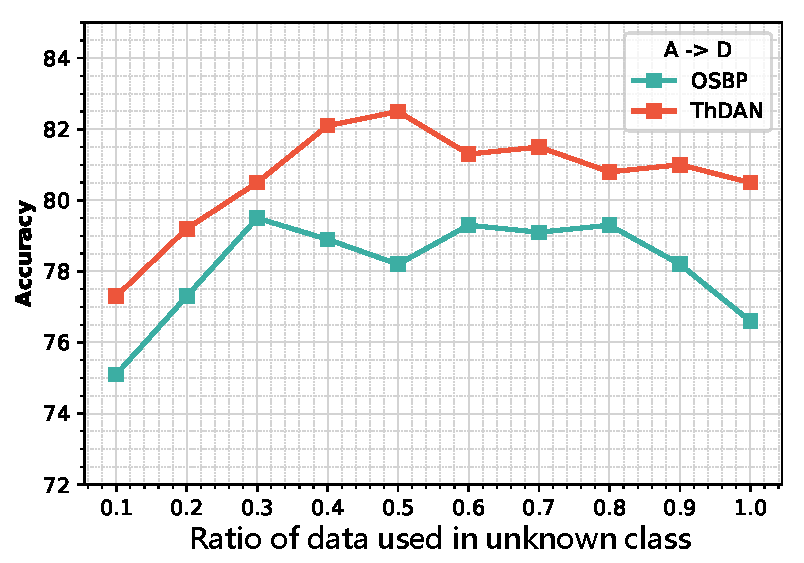
\includegraphics[width=0.34\textwidth]{contents/figures/pdf/analysis/nuknown_change.pdf} 
        \label{figure: ration of unknown}
    } 
    \subfloat[\footnotesize Accury \textit{w.r.t.} number of classes that are treated as the unknown]{
        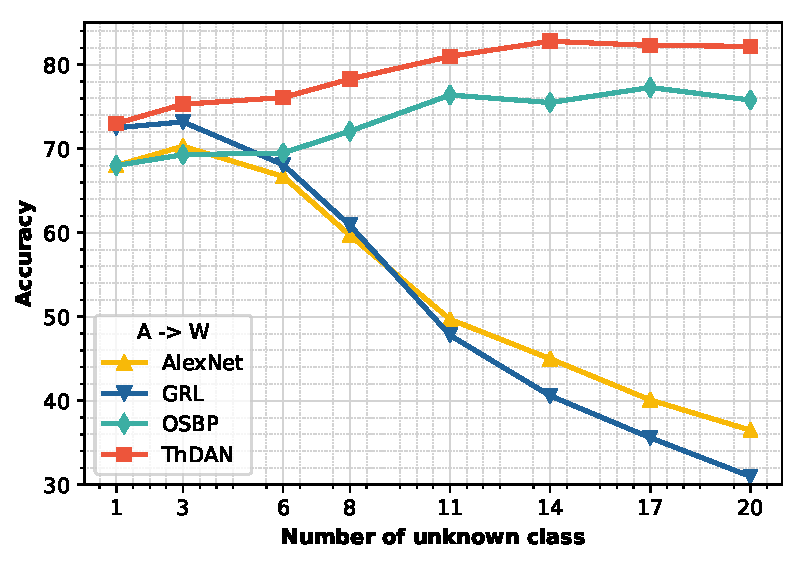
\includegraphics[width=0.33\textwidth]{contents/figures/pdf/analysis/class_change.pdf} 
        \label{figure: number of unknown class}
    }
    \subfloat[Accury \textit{w.r.t.} value of $\gamma_0$]{
        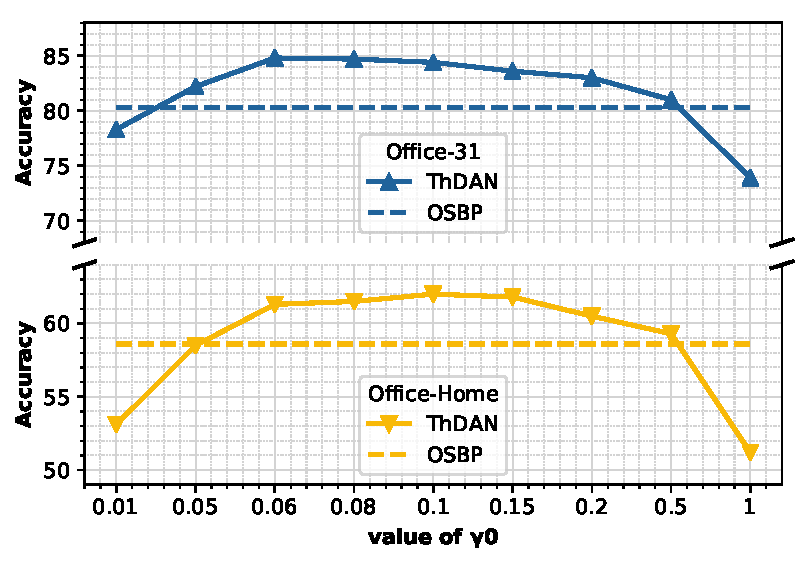
\includegraphics[width=0.33\textwidth]{contents/figures/pdf/analysis/sigma_change.pdf} 
        \label{figure: changing of sigma}
    }
    \\
    \caption{ }
    \label{figure: analysis}
\end{figure}

In the revised manuscript, the claim of it has been revised as,
\begin{siderules}
    \textit{
        \footnotesize
        (\textbf{a}): 
        The prediction accuracy of our method when we changed the ratio of unknown samples in the adaptation task \textit{A$\to$D}. 
        (\textbf{b}): 
        The prediction accuracy of our method when we changed the number of unknown classes in the adaptation task \textit{A$\to$W}. 
        (\textbf{c}): The prediction accuracy of our method when we change the value of $\sigma_0$ on dataset Office-31 and Office-Home. 
    }
\end{siderules}


\section{
    Some equations missed "," or "." at their ends.  
}

\subsection*{\underline{\textbf{Response:}}}

Thanks for pointing out the mistakes.
The equations in the revised manuscript have been corrected.




% \section*{Reference}
\bibliographystyle{elsarticle-num}
\bibliography{./reference/ref}
% \begin{thebibliography}{00}

% %% \bibitem{label}
% %% Text of bibliographic item

% \bibitem{}

% \end{thebibliography}
\end{document}
\endinput
%%
%% End of file `elsarticle-template-num.tex'.
